\message{ !name(aPilhas.tex)}\documentclass[landscape,pdftex]{jomislides}

\slidesmag{5} % escala, qto maior maiores ser�o as letras/figras/etc.

%\centerslidesfalse
\usepackage[latin1]{inputenc}
\usepackage[brazil]{babel}
\usepackage{algorithmic}
\usepackage{babel}
\usepackage{graphics}
\usepackage{color}
\usepackage{epsfig}
\usepackage{alltt,fancyvrb,amssymb}
\usepackage{listings}
\usepackage{float,ctable}
\usepackage{hyperref}

%
% Slides
% ======
%

\begin{document}

\message{ !name(aPilhas.tex) !offset(-3) }


%\input{autorHeaders}

\title{Pilhas} 
\author{Fabr�cio J. Barth}
\institution{BandTec - Faculdade de Tecnologia Bandeirantes}
\date{Fevereiro de 2011}

\SlideHeader{}
            {Disciplina de Estrutura de Dados e Armazenamento}
\SlideFooter{\theslidepartheading $\;$ --- $\;$ \theslideheading}
            {Faculdade de Tecnologia Bandeirantes \theslide}

\vpagecolor[white]{white}
\subtitle{}
\maketitle

\begin{Slide}{T�picos Principais}
  \begin{itemize}
  \item Introdu��o
  \item Interface do tipo pilha
  \item Exemplo de uso: verifica��o de express�es
  \item Implementa��o de pilha com lista encadeada
  \end{itemize}
\end{Slide}

\begin{Slide}{Introdu��o - Pilha}
  \begin{itemize}
  \item novo elemento � inserido no topo e acesso � apenas ao topo
    \begin{itemize}
      \item o primeiro que sai � o �ltimo que entrou (LIFO -
        \textit{last in, first out}) 
    \end{itemize}
   \item opera��es b�sicas:

\begin{itemize}
\item empilhar (\textit{push}) um novo elemento, inserindo-o no topo
\item desempilhar (\textit{pop}) um elemento, removendo-o do topo
\end{itemize}
   
  \end{itemize}

  \begin{center}
    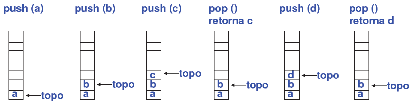
\includegraphics[width=.9\textwidth]{figuras/fig1.pdf}
  \end{center}
\end{Slide}


\begin{Slide}{Interface do tipo Pilha}
\begin{itemize}
\item 
\item 
\end{itemize}
\end{Slide}


\begin{Slide}{Estrutura com ponteiro para ela mesma}
\begin{figure}[H]
\center
\tiny
\VerbatimInput
[xleftmargin=5mm,numbers=left,obeytabs=true]{codigo/Nodo.java}
\end{figure}
\end{Slide}

\begin{Slide}{Material de \textbf{consulta}}
  \begin{itemize}
  \item Cap�tulo 11 do livro: ``Introdu��o a Estruturas de Dados'' do
    Waldemar Celes, Renato Cerqueira e Jos� Lucas Rangel.
  \end{itemize}
\end{Slide}

\begin{Slide}{Material de \textbf{refer�ncia}}
  \begin{itemize}
  \item Cap�tulo 11 do livro: ``Introdu��o a Estruturas de Dados'' do
    Waldemar Celes, Renato Cerqueira e Jos� Lucas Rangel.
  \item Imagens retiradas do site da disciplina de Programa��o II da
    PUC do Rio de
    Janeiro. \href{http://www.inf.puc-rio.br/~inf1007/}{http://www.inf.puc-rio.br/~inf1007/}. 
  \end{itemize}
\end{Slide}

\end{document}


\message{ !name(aPilhas.tex) !offset(-112) }
